\chapter{DIRC Technology}
%%History of Discovery of Cherenkov effect
DIRC detectors are based on the phenomenon of Cherenkov radiation, which was discovered by Pavel Cherenkov in 1934 and later theoretically developed by I. Frank and I. Tamm in 1937. In 1958 the three scientists shared the Nobel Prize in Physics. \cite{CherenkovHistory}.

%%Properties of Cherenkov radiation
%threshold velocity and formula
The theoretical speed limit for massive particles was postulated by Einstein to be the speed of light in a vacuum, $c = 2.99*10^9 m/s$. Particles can, however, move faster than the speed of light in an optically transparent medium, $c_{medium} = \frac{c}{n}$, where $n$ is the medium's index of refraction. When a charged particle travels through a medium with velocity greater than this so-called threshold velocity $c_{medium}$ it will emit Cherenkov Radiation. Cherenkov light has many special properties. The angle $\thetaC$ at which this radiation is emitted from the particle track is related to the particle's velocity, given by the relationship
\begin{equation}
	\cos\thetaC = \frac{1}{\beta n}
	\label{eq:cherenkovformula}
\end{equation}
This means that, for a fixed momentum, charged particles can be distinguished based purely on their Cherenkov angle. Figure \ref{fig:angleseperation} shows a comparison of the Cherenkov angle of electrons, muons, pions, kaons, and protons in fused silica ($n \approx 1.473$) as a function of particle momentum.

\begin{figure}[ht]
	\centering
	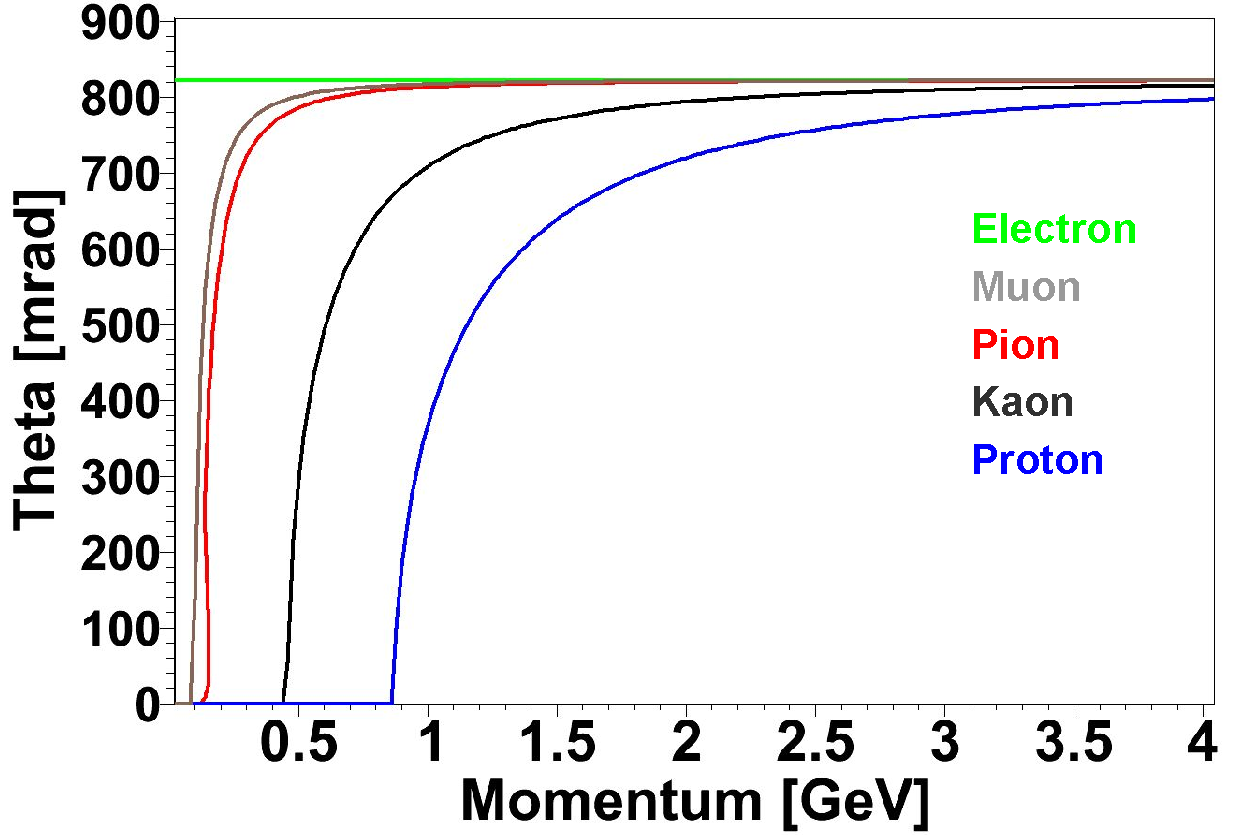
\includegraphics[scale=.7]{figures/angle_seperation.pdf}
	\caption{Particle momentum versus Cherenkov angle for different mass particles in fused silica ($n \approx 1.473$).}
	\label{fig:angleseperation}
\end{figure}

Unlike scintillation, the frequency spectrum of the emitted photons is continuous. The number of photons emitted per path length per wavelength interval is given by the Frank-Tamm formula
\begin{equation}
	\frac{\diff^2 N_{photons}}{\diff x\diff \lambda} = \frac{2\pi\alpha z^2}{\lambda(E)^2} \sin^2\thetaC(E)
	\label{eq:nphotons}
\end{equation}
where both the wavelength and Cherenkov angle are dependant on the photon energy.

%ooOOooOOooOOooOOooOOooOOooOOooOOooOOooOOooOOooOOooOOooOOooOOooOOooOOooOOooOOoo%
%ooOOooOOooOOooOOooOOooOOooOOooOOooOOooOOooOOooOOooOOooOOooOOooOOooOOooOOooOOoo%
\section{Applying the Cherenkov Effect to Particle ID}
\begin{figure}[ht]
	\centering
	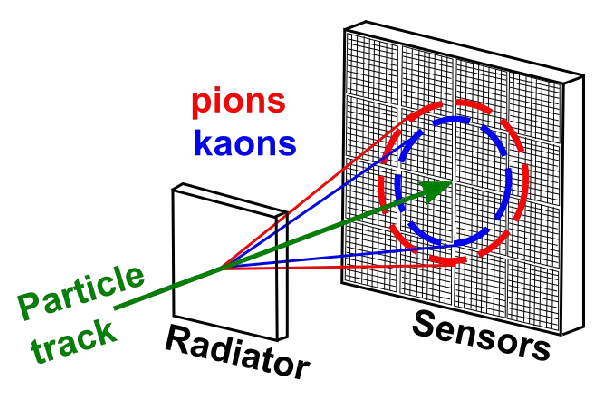
\includegraphics[scale=1]{figures/RICH.pdf}
	\caption{Typical Ring Imaging Cherenkov (RICH) detector.}
	\label{fig:richbasics}
\end{figure}

%ooOOooOOooOOooOOooOOooOOooOOooOOooOOooOOooOOooOOooOOooOOooOOooOOooOOooOOooOOoo%
%ooOOooOOooOOooOOooOOooOOooOOooOOooOOooOOooOOooOOooOOooOOooOOooOOooOOooOOooOOoo%
\section{DIRC Detectors}
The basic components of a DIRC detector are shown in Figure \ref{fig:dircbasics}.
\begin{figure}[ht]
	\centering
	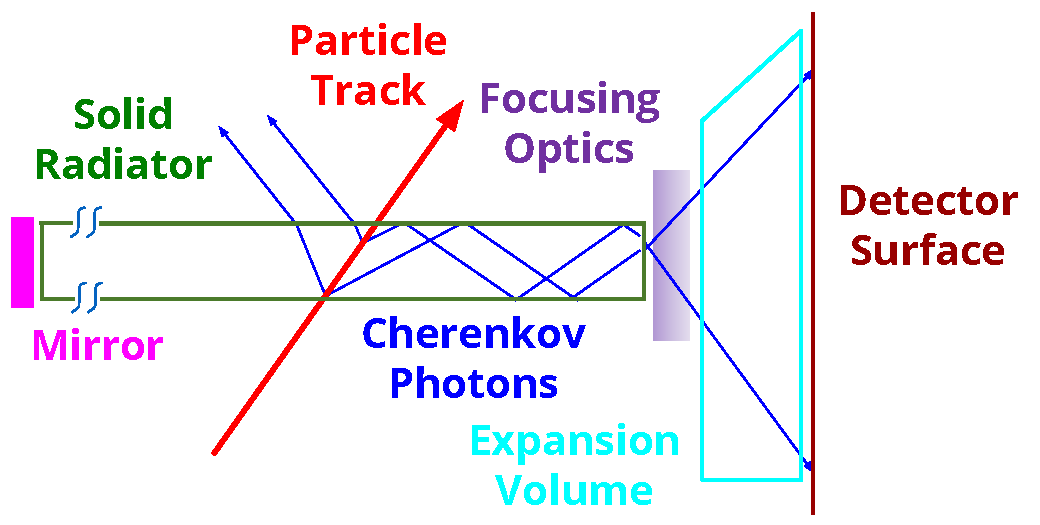
\includegraphics[scale=0.7]{figures/DIRC_components.pdf}
	\caption{The basic components of a DIRC detector: a solid radiator, typically fused silica (green); a mirror to redirect backward-going photons (pink); optional focusing optics (purple); an expansion volume to allow photons to separate in space (cyan); and a detector surface to record the position and arrival time of Cherenkov photons (maroon).}
	\label{fig:dircbasics}
\end{figure}